\begin{figure*}[t]
    \centering
    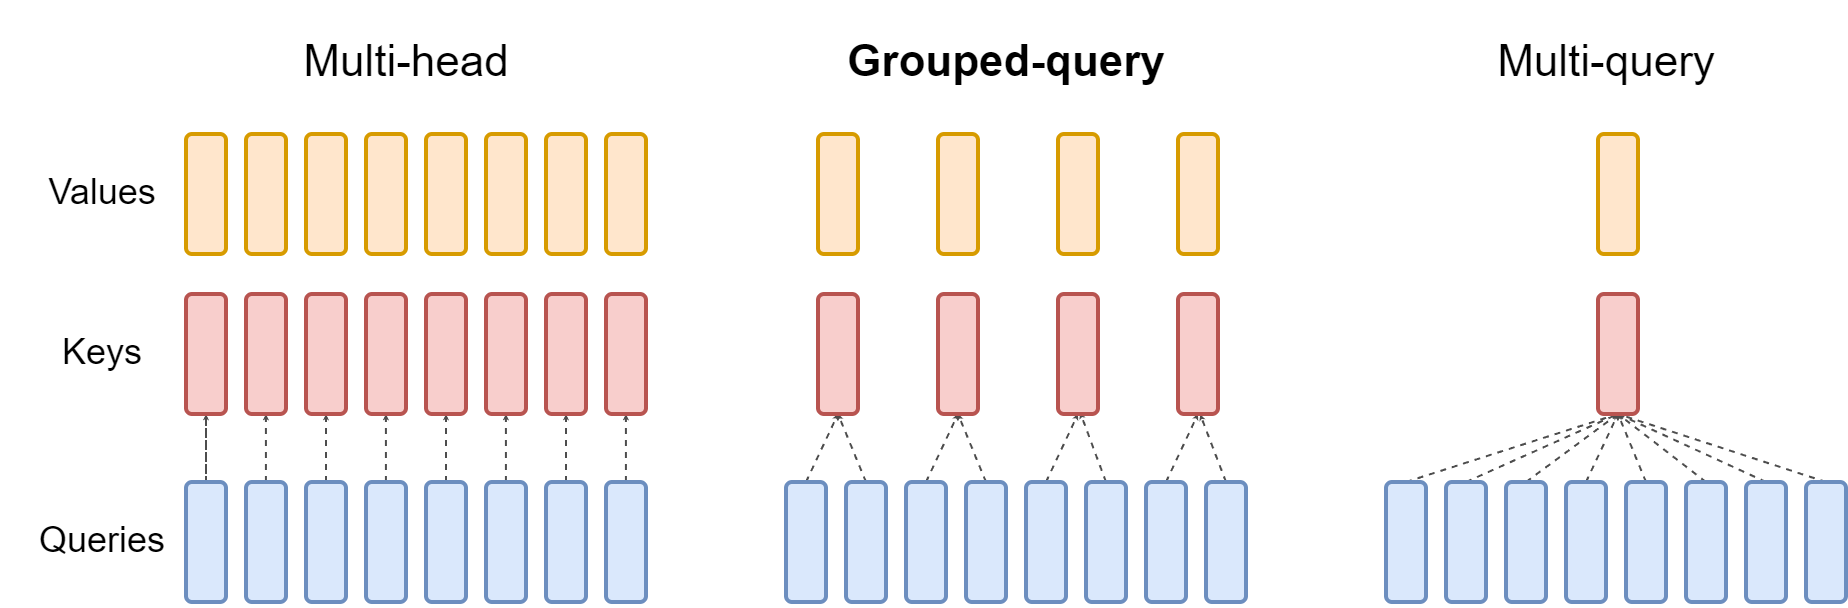
\includegraphics[width=0.9\textwidth]{images/gmq_architecture.png}
    \caption{\fullgmq 方法概览。Multi-head 注意力包含 H 个 query 头、key 头和 value 头。Multi-query 注意力在所有 query 头之间共享单个 key 头和 value 头。Grouped-query 注意力则为每个 query 头的 \emph{group} 共享单个 key 头和 value 头，从而在 multi-head 和 multi-query 注意力之间进行插值。}
    \label{fig:gmq_architecture}
\end{figure*}
